\chapter{Lecture 3}
\lhead{January 16, 2015}
\chead{21-366 Lambda Calculus Lecture 3}

\section{Left Association Deletion of Parens}
In the previous lecture, we asserted that we could take all of the parenthesis around terms which were not in argument position away without violating the uniqueness of the term. Let $X$ be a term. We define $X^*$ as the result of the left associative deletion of parenthesis from $X$. We show here what left associative deletion looks like for various terms. Later, in our uniqueness proof, we will refer back to these example terms.\\

\begin{eqnarray*}
  (1) &=& x\\
  (2) &=& (\l x_1 \ldots x_n . x_i)\\
  (3) &=& (\l x_1 \ldots x_n.((\l xX_0)X_1) \ldots )X_m))\\
  (4) &=& (\underbrace{\l x_1 \ldots x_n}_{\hbox{Lambda prefix}} . \underbrace{(( \ldots (\underbrace{x_i}_{\hbox{head}} X_i) \ldots )X_m )}_{\hbox{matrix}}\\
\end{eqnarray*}

\margnot{Illustration of 3 and 4}{
\begin{center}
  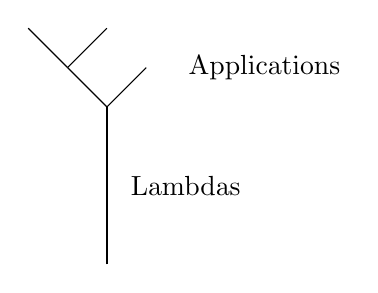
\begin{tikzpicture}
    \draw (0,0) -- (0,2);
    \draw (0,2) -- (.5, 2.5);
    \draw (0,2) -- (-.5, 2.5);
    \draw (-0.5, 2.5) -- (-1, 3);
    \draw (-0.5, 2.5) -- (0, 3);

    \draw (1,1) node {Lambdas};
    \draw (2,2.5) node {Applications};
  \end{tikzpicture}
\end{center}
}

Left association deletion for case $(1)$ is trival. There are no parenthesis at all, so we delete nothing. In case $(2)$, we have a sequence of lambdas followed by a single application. This does not have any parenthesis around subterms which are not in argument position, so again we cannot delete any parenthesis. Case $(3)$ is the first case where we can delete something. The term at the head of the application is of the form $((\l xX_0)X_1)$, which can be reduced to $(\l xX_0X_1)$. In case 4, the first subterm is of the form $((x_i X_i)\ldots)$. The innermost parens here can be removed, giving another term which has parenthesis around the subterm not in argument position. By repeating this process, $(4*)$ is derived.

\begin{eqnarray*}
  (1*) &=& x\\
  (2*) &=& (\l x_1\ldots x_n.x_i)\\
  (3*) &=& (\l x_1 \ldots x_n . (\l xX_0X_1 \ldots X_m)\\
  (4*) &=& (\l x_1 \ldots x_n . x_LX_1 \ldots X_m)\\
\end{eqnarray*}

\subsection{Proof of Uniqueness}
Our claim is that $X \not= Y$ if and only if $X^* \not= Y$. There are four possible cases for the form of our terms $X$ and $Y$. We will prove the claim by induction on $X$. Our base case is $X$ as a variable. It is either of the form $((x)y)$ or $(x(y))$, or a single variable $z$, where $x, y$ and $z$ could have subterms.\\

Our first case is that $X := z$. It has no parens, so we are done. If it is of the form $((xy)z)$ or $(x(yz))$, however, we can evaluate $((xy)z)*$ and $(x(yz))*$:
\begin{eqnarray*}
  ((xy)z)* &=& xyz\\
  (x(yz))* &=& x(yz)\\
\end{eqnarray*}
We can say that we can uniquely restore the parens, based on whether we are in the first or second listed case.\\

Induction Step: In case (2), we have two parens. This can only happen the two parens are the outermost parens around the term:
\begin{equation*}
  (\l x_1 \ldots x_n.X_{i_1}\ldots X_{i_k})
\end{equation*}
In our left association deletion scheme, we do not delete outermost parens, so the term remains unchanged. If all of the variables can be uniquely restored, then case $(2)$ can be uniquely restored as well.\\

$X^* = Y^*$ in cases where $(1)^*, (2)^* \Rightarrow X = Y$.\\

Consider the proper pairing of parens. Case (2) applies to $X$ implies (2) applies to $Y$ and case (3) applies to $X$ implies (3) applies to $Y$.
\begin{equation*}
  (\l x_1 \ldots x_n (\l xX_0))(\ \ \ )(\ \ \ ))
\end{equation*}
The parens in argument position must be reconstructable by the induction hypothesis. FIGURE OUT AND FIX THIS PROOF.

\section{Substitution of a Term for a Variable}
A problem arises when we attempt to substitute one term into another where both terms contain the same variables. The problem is that it is ambiguous which variables mean what when both are represented by the same symbol. Take for example the following application:
\begin{eqnarray*}
  (\l x . yx)(zx)\\
  (\l x . y(zx))\\
\end{eqnarray*}
When we make this application, we have $x$s both before and after the application, but the $x$s mean different things. In this simplified example, it can be figured out what is going on by manual inspection, but it gets worse when the terms are more complicated. We therefore have an incentive to resolve this naming issue before then. An easy solution is to simply change the name of the symbol in the lambda:
\begin{eqnarray*}
  (\l u . yu)\\
  (\l u . (zx)u)
\end{eqnarray*}
TODO: THIS IS WRONG. WHY.

\subsection{Clash Graphs}
\index{Clash Graph|textbf}
We have some abstract term. From the root, there is only one path to any given leaf.
\begin{center}
  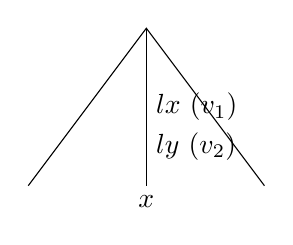
\begin{tikzpicture}
    \draw (0,0) -- (0,-1) node[anchor=west] {$\l x\ (v_1)$};
    \draw (0,-1) -- (0,-2) node[anchor=north] {$x$};
    \draw (-1.5,-2) -- (0,0) -- (1.5,-2);

    \draw (0,-1.5) node[anchor=west] {$\l y\ (v_2)$};

    % Draw an arrow from x to \l x.
  \end{tikzpicture}
\end{center}

We define a \textbf{clash graph} which has verticies that are the \l{} abstraction nodes of the term. $v_1$ is adjacent to $v_2$ provided that $v_2$ lies on the path from $v_1$ to a leaf which it binds, or vice versa.
